\taskpic { Трубка в форме ромба с одинаковыми сторонами и закругленными
  углами расположена в вертикальной плоскости, как показано на
  рисунке. Один раз шарик скатывается в трубке по сторонам $AB$ и
  $BC$, а другой раз по сторонам $AD$ и $DC$. В каком случае он
  скатится быстрее? }
{
  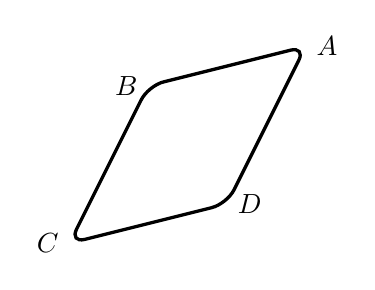
\begin{tikzpicture}
    \draw[very thick,rounded corners=0.2cm] (1,2) node[left] {$B$} --
    (3,2.5) node[right] {$A$}  -- (2,0.5) node[right] {$D$} -- (0,0)
    node[left] {$C$}  -- cycle;  
  \end{tikzpicture}
}
% Шаскольская-Эльцин, 2.6